%!TEX root = ./main.tex
%   
% @author Lawrence Cabac
% @date   March 2006
% 
%%%%%%%%%%%%%%%%%%%%%%%%%%%%%%%%%%%%%%%%%%%%


\documentclass[10pt,a4paper]{llncs}

\usepackage{ngerman}
\usepackage[utf8]{inputenc}
\usepackage{rotating}
\usepackage[dvips]{epsfig}
\usepackage{graphicx}
\usepackage{acronym}
\usepackage{index}


\usepackage[T1]{fontenc}

\usepackage{hyperref}  
%\usepackage[pagebackref]{hyperref}  

\date{\today}
\newcommand{\netscale}{.75}
\pagestyle{myheadings}
\setcounter{tocdepth}{2}
%!TEX root = ./aose.tex
%%%%%%%%%%%%%%%%%%%%%%%%%%%%%%%%%%%%%%%%%%%%%%%%%%
%------------- MulanCapaIntegration MAKROS ---------------------
%%%%%%%%%%%%%%%%%%%%%%%%%%%%%%%%%%%%%%%%%%%%%%%%%%

\newcommand{\loadNetMec}{loadNet-mechanism}
\newcommand{\loadNet}{loadNet}
\newcommand{\muca}[1]{mulanCapa:#1}
\newcommand{\mucaImg}{../MulanCapaIntegration/images}

%%%%%%%%%%%%%%%%%%%%%%%%%%%%%%%%%%%%%%%%%%%%%%%%%%
%------------- COMMON MAKROS ---------------------
%%%%%%%%%%%%%%%%%%%%%%%%%%%%%%%%%%%%%%%%%%%%%%%%%%
\newcommand{\Capa}{{\sc Capa}}
\newcommand{\capa}{{\sc Capa}}
\newcommand{\Mulan}{{\sc Mulan}}
\newcommand{\mulan}{{\sc Mulan}}
\newcommand{\Renew}{{\sc Renew}}
\newcommand{\renew}{{\sc Renew}}
\newcommand{\Pasoe}{{\sc Pasoe}}
\newcommand{\pasoe}{{\sc Pasoe}}

\newcommand{\postit}[1]{\marginpar{{\parbox{\linewidth}{\footnotesize\textsf{{\color{red}#1}}}}}}
\newcommand{\zitat}[1]{``#1''}

%%%use : \image{<PATH>/<image-name>}{<Caption>}{<project-name>:<label>}
\newcommand{\image}[3]{
\begin{figure}[!htb]
\centering
	\includegraphics[width=\textwidth]{#1}
  \caption{#2}
  \label{fig:#3}
\end{figure}
}%


%---------- Index erstellen ------------
\makeindex
%---------------------------------------

\begin{document}

%%%%%%%%%%%%%%%%%%%%%%%%%%%%%%%%%%%%%%%%%%%%%%%%%%
%------------- TITEL ---------------------------
%%%%%%%%%%%%%%%%%%%%%%%%%%%%%%%%%%%%%%%%%%%%%%%%%%

      
\title{Projektabläufe und Scheduling}
\titlerunning{Scheduling}      

\author{Louis Kobras}

\institute{Department  Informatik, TGI, University of Hamburg\\
   http://www.informatik.uni-hamburg.de/TGI/%% hier lieber email adressen
 }
\institute{\href{http://www.informatik.uni-hamburg.de/TGI/}{Fachbereich Informatik, TGI, Universität Hamburg}}
      

%%%%%%%%%%%%%%%%%%%%%%%%%%%%%%%%%%%%%%%%%%%%%%%%%%%
%------------- DOCUMENT -------------------------
%%%%%%%%%%%%%%%%%%%%%%%%%%%%%%%%%%%%%%%%%%%%%%%%%%%

% Bitte nur die englische oder nur die deutsche Fassung im Hauptverzeichnis einbinden. 

\newpage
%Deutsche Fassung:
%!TEX root = ./main.tex
   
% @author Lawrence Cabac
% @date   November 2007
% 
%%%%%%%%%%%%%%%%%%%%%%%%%%%%%%%%%%%%%%%%%%%%


%%%%%%%%%%%%%%%%%%%%%%%%%%%%%%%%%%%%%%%%%%%%%%%%%%
%------------- TITEL ---------------------------
%%%%%%%%%%%%%%%%%%%%%%%%%%%%%%%%%%%%%%%%%%%%%%%%%%

      
%% Please replace the following and remove the brackets (<,>)
\title{Projektstrukturierungstechniken}
\titlerunning{Strukturierungstechiken}

\author{Louis Kobras}

\institute{\href{http://www.informatik.uni-hamburg.de/TGI/}{Fachbereich Informatik, TGI, Universität Hamburg}}
      

%%%%%%%%%%%%%%%%%%%%%%%%%%%%%%%%%%%%%%%%%%%%%%%%%%%
%------------- DOCUMENT -------------------------
%%%%%%%%%%%%%%%%%%%%%%%%%%%%%%%%%%%%%%%%%%%%%%%%%%%


\renewcommand{\textfraction}{0}

\maketitle
\tableofcontents


\selectlanguage{ngerman}
\begin{abstract}
	Diese Arbeit beschäftigt sich mit Techniken und Vorgehensweisen zur Strukturierung von Softwareentwicklungsprojekten.
	\index{abstract}
	Es werden hierbei mit Hinblick auf die Evolution der Softwareentwicklung von einer Ingenieurswissenschaft zur eigenständigen Profession Techniken aus dem Projektmanagement sowie Verfahren aus der agilen Softwareentwicklung vorgestellt, mit deren Anwendung moderne Softwareentwicklungsprojekte durchgeführt werden.
	

\end{abstract}
%\newpage
\section{Motivation}
	\label{sec:motivation}
	Das effiziente Entwickeln von Software ist ein Problem, welches die Fachwelt seit Beginn der Softwareentwicklung selbst beschäftigt.
	Hierfür wird sich seit jeher verschiedenen Techniken entwickelt, die aus anderen Fächern, wie beispielsweise dem Ingenieurswesen oder dem Proiektmanagement, entlehnt oder komplett übernommen wurden.
	
	Ziel dieser Arbeit ist es, einige dieser Techniken zu untersuchen und darzustellen, was in der heutigen Zeit Standart in der Softwareentwicklung ist.
	
	
\section{Einführung}
	\label{sec:introduction}
	Auch bei Softwareentwicklung handelt es sich um Projekte verschiedener Größenordnung.
	Deswegen ist es nicht verwunderlich, Strukturierungstechniken zu sehen, die bei Bauprojekten oder auch in der Wirtschaft beim Pizza backen \footnote{
		\url{http://www.criticalpathmethod.net/Critical-Path-Method-Example.html}
	} angewandt werden.
	
	Über das letzte Jahrhundert, während Software am Entstehen war, hat sich auch die Entwicklungspraxis stets verändert.
	Es gibt verschiedene Techniken, um Software zu entwickeln, die ihrer Zeit stets angemessen sind.
	Ebenso gibt es verschiedene Möglichkeiten, den Entwicklungsprozess zu strukturieren, welche sich analog zu den Entwicklungstechniken gewandelt haben.
	So ist zum Beispiel die dokumentationslaste Programmiersprache FORTRAN begleitet worden vom starren Wasserfallentwicklungsmodell, während heutige Sprachen deutlich einfacher von der Hand gehen und gleichsam Projekte in diesen begleitet werden von flexiblen, agilen, Entwicklungstechniken, wie sie unter Anderem in Scrum und eXtreme Programming verwendet werden.
	
	Die heutigen Techniken zur Strukturierung können aufgeteilt werden in \textit{Langzeitstrukturierung} und \textit{Kurzzeitstrukturierung}, wobei die Langzeitstrukturierung ein gesamtes Entwicklungsprojekt darzustellen und zu leiten vermag, während die Kurzzeitstrukturierung besser geeignet ist, um einzelne Abschnitte innerhalb eines Projektes, so genannte \textit{Sprints}, zu organisieren und zu koordinieren.
	
	Es muss jedoch erwähnt werden, dass sich die hier beschriebenen Techniken selbstverständlich auf beide Strukturierungsebenen anwenden lassen.
	
	Die Techniken, die in dieser Arbeit beschrieben werden, sind allgemeingültig derart, dass sie für Projekte verschiedener Art, nicht nur der Softwareentwicklung, verwendet werden können.
	Dies bedeutet auch, dass sie nicht auf die Entwicklung von bestimmten Arten von Software beschränkt sind.
	So lässt sich mit diesen Techniken zweifelsfrei eine verteilt laufende Software entwickeln, und unter Zuhilfenahme von Web-Diensten wie einem serverseitigen Zeitplan oder Cloud-Diensten durchaus auch verteilte Entwicklung von Software betreiben.
	
	Es wird nun zunächst einen historisch-evolutionären Überblick über die Softwareentwicklung an sich geben, bevor drei (miteinander verwandte) Langzeitstrukturierungstechniken und zwei Kurzzeitstrukturierungstechniken vorgestellt werden, die in der heutigen Softwareentwicklung praktisch betrieben werden.
	
\section{Geschichte der Softwareentwicklung}
	\label{sec:history}
	Obwohl Softwareentwicklung im Vergleich zur Geschichte beispielsweise der Mathematik eine junge Profession ist, hat sie doch viel Wandel erfahren, seitdem erste vollautomatische Rechner von IBM in den 1940er Jahren\footnote{
		\url{http://www-03.ibm.com/ibm/history/history/year_1944.html}
	} oder noch früher die ersten Computerprogramme im 19. Jahrhundert von Ada Lovelace geschrieben wurden.

	Softwareentwicklung, nach dem englischen Begriff ``Software Engineering'', wurde ursprünglich wie eine Ingenieurswissenschaft behandelt\footnote{
		\url{https://sewiki.iai.uni-bonn.de/teaching/labs/xp/2009b/seminar/history}
	}.
	Dies jedoch war ein suboptimaler Ansatz.
	\subsection{Anfänge im Wasserfallmodell}
		\label{ssec:waterfall}
		Ähnlich wie im Bauingenieurswesen wurde bei der Softwareentwicklung zunächst der so genannte Wasserfallansatz verfolgt.
		
		Bei diesem folgt eine festgelegte Phase der Nächsten, und ein Zurückgehen in eine bereits abgeschlossene Phase war zwar theoretisch möglich und vom Entwickler sogar gehofft\footnote{
			http://www.cs.umd.edu/class/spring2003/cmsc838p/Process/waterfall.pdf
		}, praktisch jedoch selten umzusetzen\footnote{
			\url{http://techbeacon.com/agility-beyond-history\%E2\%80\%94-legacy\%E2\%80\%94-agile-development}
		}.
		\begin{figure}[ht!]
			\begin{center}
				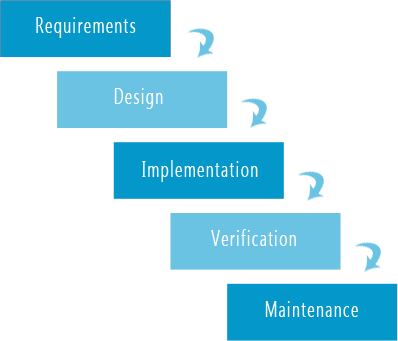
\includegraphics[scale=.4]{images/waterfall.png}
			\end{center}
			\caption{Darstellung des Wasserfallmodells. Die Phasen werden strikt hierarchisch abgearbeitet.}
			\label{img:waterfall}
		\end{figure}\\
		Im Ingenieurswesen, also dem Ursprung des Wasserfallmodells, ist dieses durchaus sinnvoll, da Baustoffe teuer sind und minimale Abweichungen katastrophale Folgen haben können.
		Bei Software jedoch ist der Unterschied vehement: Baustoffe haben keine Zusatzkosten, und kleine Fehler kosten keine Menschenleben.
		Desweiteren wird der Bedarf für eine Eisenbahnbrücke sich nicht ändern über einige Jahre - die Anforderungen an Software schon.
		
		Dies stand im Konflikt mit der Tatsache, dass Softwareprojekte nahezu grundsätzlich sowohl ihren zeitlichen als auch ihren finanziellen Rahmen sprengten.
		Die Ansicht, dass mehr Zeit in Planung dazu führe, weniger und besseren Code zu schreiben, mag korrekt sein, jedoch änderten sich die Anforderungen rasant und die Planung, einmal abgeschlossen und überführt in Umsetzung, war nicht in der Lage, auf dieses Änderungstempo angemessen zu reagieren.
		\\\\
		Das Wasserfallmodell differenziert zwischen fünf bis sieben Phasen, je nach Quelle.
		Die originale Beschreibung von Royce 1970\footnote{
			\url{http://www.cs.umd.edu/class/spring2003/cmsc838p/Process/waterfall.pdf Seite 2}
		} liefert sieben: Systemanforderungen, Softwareanforderungen, Analyse, Design, Implementation, Test, Betrieb.
		
		Der Anteil der Zeit am eigentlichen Schreiben von Quellcode wird damit effektiv minimiert, auf etwa ein Drittel des Projektumfangs.\footnote{
			\url{http://www.oxagile.com/company/blog/the-waterfall-model/}
		}
		Da jedoch ein Softwareprojekt lebendig ist, ist Zeit, die mit Planung verbracht wurde, möglicherweise nicht angemessen investiert, denn die Anforderungen können sich ohne Vorankündigung ändern.
		
		Gegeben ein statisches Umfeld ist dieser Ansatz jedoch hervorragend, denn die meisten möglichen Fehlerfälle werden noch vor der eigentlichen Implementation erkannt und behandelt, sodass die Kosten durch spätere Korrekturen minimiert werden.
		
	\subsection{Aufsteigen flexibler Modelle}
		\label{ssec:flexible}
		In den 90er Jahren begann die Idee der Flexibilität sich durchzusetzen.
		Nachdem noch 1995 zu viele Ressourcen bei Softwareprojekten verloren gingen,\footnote{
			\url{http://www.techrepublic.com/blog/tech-decision-maker/the-roots-of-agile-project-management/}
		} etwa drei Viertel aller Software entwickelt im Auftrag des us-amerikanischen Verteidigungsministeriums wurde entweder nicht genutzt oder während der Entwicklung terminiert, nur zwei Prozent der Software war beim Ausliefern so benutzbar wie gedacht, wurde mehr und mehr Rücksicht auf Flexibilität genommen.
		
		Es wurde das Prototyping eingeführt, bei dem ein billiger Prototyp der Software dem Auftraggeber vorgelegt wurde, um anhand dessen eine Rückmeldung über die Verwendbarkeit der Software zu erhalten.
		
		Dies wurde weitergeführt in das Spiralmodell, bei dem stets ein überarbeiteter Prototyp vorgelegt wurde, um so immer weiter feinabstimmen zu können.
		
		Analog dazu kam die Entwicklung von kleinen Zwischenabgaben statt der einen Projektfertigstellung.
		Komponenten wurden ausgeliefert, wenn sie fertig waren, und die Software wurde so erweitert, während sie schon in Benutzung war.
		Der Höhepunkt dessen ist die iterative Entwicklung, bei der Auftraggeber funktionierende Software testen und bewerten können, die daraufhin überarbeitet und wieder vorgelegt wird.
		
		Diese Iteration trat über von der Auslieferung der Software in die Entwicklung, und es entstand ein iterativ-inkrementeller Entwicklungsprozess.
		
		Über die 80er und 90er Jahre enstanden die beiden heute am weitesten verbreiteten Entwicklungspraktiken: \textit{Scrum} und \textit{eXtreme Programming}.
		
	\subsection{Kulmination: Das Agile Manifest}
		\label{ssec:agile}
		
		Diese Entwicklungspraktiken haben sich bewährt und sowohl für Kostenreduktion als auch für erhebliche Zeitersparnis und somit zu erhöhter Kundenzufriedenheit geführt.
		Was fehlte war ein geeigneter Sammelbegriff und eine Festlegung der Grundprinzipien der neuen Art der Softwareentwicklung.
		
		2001 in Utah trafen sich Vorreiter der zu der Zeit als \textit{light} bezeichneten Softwareentwicklung (im Gegensatz zur \textit{heavyweight}-Entwicklung im Wasserfallmodell).
		Ihr Ziel war es, die Prinzipien, nach denen sie arbeiteten, auszuformulieren und einen Namen zu finden, mit dem sie einverstanden waren.
		
		Sie schufen das \textit{Agile Manifest}\footnote{
			\url{http://agilemanifesto.org/}
		}, eine Festlegung von vier Grundsätzen und zwölf Prinzipien, als Konsens von allen Anwesenden, unter Anderem Ken Schwaber und Jeff Sutherland, den Entwicklern von Scrum, und Jim Highsmith, den Entwickler der \textit{Adaptiven Softwareentwicklung}.
		Am 13. Februar 2001 wurde das Manifest erstmalig von den 17 anwesenden Vorreitern der nun \textit{agil} getauften Methodiken unterschrieben, wobei es explizit der Reaktion auf Änderungen Vorzug gibt über dem Folgen eines starren Plans.		
		
\section{Langzeitstrukturierung von Projekten}
	\label{sec:long-term}
	In diesem Abschnitt wird die Struktur des gesamten Projektes über seine komplette Dauer behandelt.
	
	Eine derartige Übersicht ist sinnvoll, um einerseits einen Überblick über vorhandene und gebundene Ressourcen wie Teammitglieder oder schlicht Zeit zu erhalten und andererseits die größeren Zusammenhänge und Abhängigkeiten einzelner Tasks nicht aus den Augen zu verlieren.
	
	Ein Strukturplan des Projektes, der sich über die komplette Dauer von Beginn bis Deadline erstreckt, macht es einfacher, zu beurteilen, ob sich ein Projekt noch im Zeitplan befindet.
	Ebenso ermöglicht es einen Vergleich des Kurses des Projektes mit den aktuellen Zielsetzungen und somit ein frühes Gegensteuern, sollte das Projekt von den Vorgaben abzuweichen drohen.
	
	Es werden nun im Folgenden drei Techniken vorgestellt werden, mit deren Hilfe sich ein Überblick über den gesamten Projektstatus erlangen lässt.
	Es ist anzumerken, dass es sich hierbei nicht um Softwareentwicklungstechniken, sondern um Projektmanagementtechniken im Allgemeinen handelt, die sich jedoch ohne weiteres auf Softwareentwicklung anwenden lassen.
	\subsection{Critical Path Method}
		\label{ssec:critical}
		\begin{figure}[ht]
			\begin{center}
				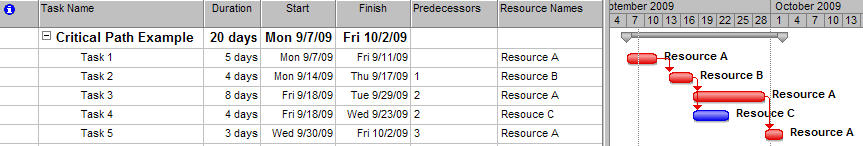
\includegraphics[width=\textwidth]{images/critical-path.jpg}
			\end{center}
			\caption{Critical Path-Diagramm, erstellt mit Microsoft Project. Links die Projektdaten, rechts das eigentliche Diagramm, Critical Path in rot. Diese Abbildung ist gleichzeitig auch ein Gantt-Diagramm, siehe unten.}
			\label{img:crit}
		\end{figure}
		Die erste untersuchte Methode zur Langzeitprojektanalyse ist die Critical Path Method (CPM).
		Sie entstand in den 1950ern als Projektmanagementwerkzeug zur Konstruktion von Chemiefabriken in den USA, wo sie der verwendenden Firma allein im ersten Jahr eine Million US-Dollar einsparte\footnote{
			\url{http://www.criticalpathmethod.net/}
		}.
		Beim Critial Path handelt es sich um den kürzestmöglichen Pfad durch ein Projekt, also die Kette von Aufgaben, die nacheinander ausgeführt werden müssen, um das Projekt zu vervollständigen.
		
		Grundsätzlich werden hierbei sämtliche Aufgaben mit ihren Bearbeitungszeitanforderungen und Abhängigkeiten in einem Flow Chart angeordnet derart, dass jede Aktivität und Aktivitätenkette sowie deren erwartete Zeit dargestellt werden.
		Aus diesem Flow Chart kann der kritische Pfad abgelesen werden.
		Es wird immer ein frühestmöglicher Fertigungszeitpunkt für einzelne Aufgaben und ein recht später bestimmt, wobei beim späteren Fertigungszeitpunkt auf wahrscheinliche Ausnahme- und Fehlersituationen Rücksicht genommen wird (worst-case scenario).
		
		\subsubsection{Critical Path Analysis (CPA).}
			\label{sssec:cpa}
			Jeder Aufgabe wird eine Dauer zugewiesen.
			Die Tasks werden in eine Parent-Child-Relation gesetzt, wodurch ein gerichteter Graph entsteht.
			Die Zeiten aller Pfade durch den Graphen werden addiert.
			Der Pfad mit der längsten Zeit ist der Critical Path.
			Alle anderen Pfade können parallel dazu bearbeitet werden.
		\subsubsection{Drag und Float.}
			\label{sssec:drag}
			\textbf{Drag} tritt ein, wenn ein so genanntes kritisches Element, ein Element des kritischen Pfades, verzögert oder unterbrochen wird.
			Dieses Element zieht dann (engl. \textit{drag}) das gesamte Projekt in die Länge.
			\textbf{Float} ist die Bezeichnung für den zeitlichen Spielraum eines Elementes, bevor es zum Drag kommt (Fehlertoleranz).
			Subkritische Elemente, Elemente, die nicht zum Critical Path gehören, haben einen \textit{total float}, da ihre Verzögerung das Projekt aufgrund der Parallelisierung nicht verzögert.
			
			Es sollte stets darauf geachtet werden, genug Float in die Planung mit einzubeziehen.
			
		\subsubsection{Vorteile der CPM.}
			\label{sssec:cpm-pro}
			Als Vorteil lässt sich sagen, dass CPM die Produktivität und die Effizienz eines Entwicklerteams erhöht und Unsicherheiten in Hinsicht auf den zukünftigen Zustand des Projektes minimiert werden, wodurch insgesamt die Wahrscheinlichkeit erhöht wird, die Deadline zu treffen.
			
			Da zur Erstellung bereits ein minimaler und ein maximaler Zeitverbrauch sowie wahrscheinliche Störfälle einkalkuliert wurden, wird der Zeitplan von einzelnen Ausnahmen nicht nennenswert belastet und es kann darauf reagiert werden, ohne mit schwerwiegenden Konsequenzen für den Rest des Projektes rechnen zu müssen.
			
			Ebenso ist hierbei im Vorfeld bekannt, wo es zu Ressourcenengpässen kommen kann und wann welche Ressourcen gebraucht werden. Dies ermöglicht es, frühzeitig dafür zu sorgen, dass alle benötigten Ressourcen zur Verfügung stehen.
			
			Als \textbf{Nachteil} lässt sich jedoch sagen, dass ein Critical Path bei komplexen Projekten schnell unübersichtlich wird und Berechnungsfehler oder ausnehmend viele Störfälle dazu führen können, dass der vom Critical Path vorgegebene Zeitraum nicht eingehalten werden kann.
			Desweiteren kann unter Umständen viel micromanagement erforderlich sein, um alle Forderungen des Critical Path zu erfüllen.
			
			
	\subsection{PERT (Program evaluation and review technique)}
		\label{ssec:pert}
		\begin{figure}[ht]
			\begin{center}
				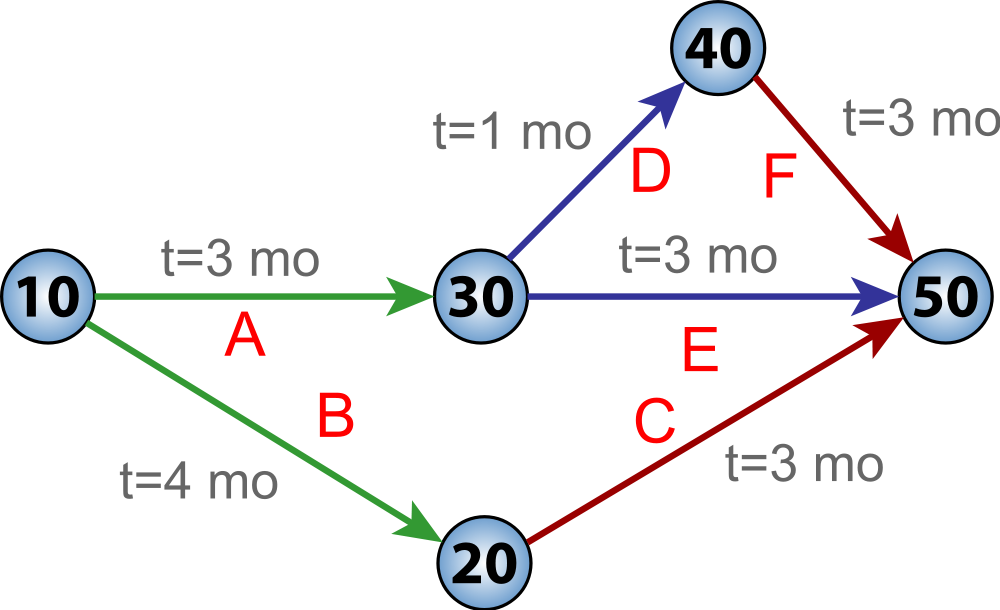
\includegraphics[scale=.2]{images/pert.png}
			\end{center}
			\caption{PERT-Diagramm für ein 7-Monate-Projekt mit 5 Milestones (10-50), 6 Aktivitäten (A-F)}
			\label{img:pert}
		\end{figure}
		PERT ist eine Technik ähnlich zur Critical Path Method, die in relativer zeitlicher Nähe entstanden ist und ursprünglich von der US-Navy entwickelt wurde zur Risikoabschätzung bei einem Programm zur Bestückung von U-Booten mit Nuklearwaffen\footnote{
			\url{http://www.academia.edu/11933878/PERT_The_Polaris_Missile_Project_Case}
		}, genannt Polaris\footnote{
			\url{http://www.criticalpathmethod.net/}
		}.
		
		PERT ist eine analytischere Alternative zur bereits beschriebenen Critical Path Method, bei der davon ausgegangen wird, dass die Zeitanforderungen für einen Task zwischen seiner Minimalanforderung und seiner Maximalanforderung zufallsverteilt sind (nach der Beta-Verteilung, deren Erläuterung hier zu weit ausufern würde).
		
		Es wird unterschieden zwischen \textit{Milestones} und \textit{Aktivitäten}, wobei immer eine Aktivität zwei Milestones verbindet, ein Milestone ein zu erreichendes Ziel im Projekt ist und eine Aktivität die Umsetzung dieses Ziels, gegeben alle Vorbedingungen.
		
		Die erwartete Zeit einer Aktivität lässt sich approximieren durch die Formel\footnote{
			\url{https://www.mindtools.com/critpath.html}
		}
		\begin{equation}
			E = \frac{B + 4 \cdot A + W}{6},
		\end{equation}
		wobei \textit{E} die zu erwartende Dauer einer Aktivität ist, \textit{B} die kürzestmögliche Zeit (\textit{best case}), \textit{A} die durchschnittliche Zeit (\textit{average case}) und \textit{W} die längstmögliche Zeit (\textit{worst case}).
		
		Aktivitäten bei PERT berücksichtigen also die Extremfälle, gehen aber davon aus, dass diese seltener auftreten als ein Normalfall (auf einen Extremfall kommen zwei Normalfälle).
		Diese Zeiten werden gemittelt und ergeben die zu erwartende Dauer einer jeden Aktivität.
		
		Das Verfahren ist ähnlich zur Critical Path Method, indem zuerst die Milestones und Aktivitäten (Tasks und Subtasks) definiert\footnote{
			\url{http://www.netmba.com/operations/project/pert/}
		} und diese sequenziell angeordnet und in ein Netzdiagramm überführt werden.
		Anschließend werden für die einzelnen Aktivitäten die Zeiten berechnet und es lässt sich der kritische Pfad aus dem Diagramm ablesen.
		
		Das Diagramm kann stetig aktualisiert werden, um so Verschiebungen im Zeitplan aufzuzeigen.
		
		\subsubsection{Vorteile.}
			\label{sssec:pert-pro}
			PERT, wie auch die Critical Path Method, gibt die erwartete Fertigstellungszeit an.
			Ebenso kann man direkt die Start- und Endzeiten von Tasks einsehen.
			
			PERT gibt eine gute Übersicht über Abhängigkeiten und lässt die Projektdaten gut darstellen.
			
		\subsubsection{Nachteile.}
			\label{sssec:pert-con}
			Die Zeitschätzung ist subjektiv.
			
			Durch Fehleinschätzungen und Verzögerungen auf einem Nebenpfad kann dieser Pfad zu einem neuen kritischen Pfad werden.
			
			Auch PERT-Diagramme können schnell unübersichtlich werden.
			
	\subsection{Gantt-Diagramme}
		\label{ssec:gantt}
		\begin{figure}[ht]
			\begin{center}
				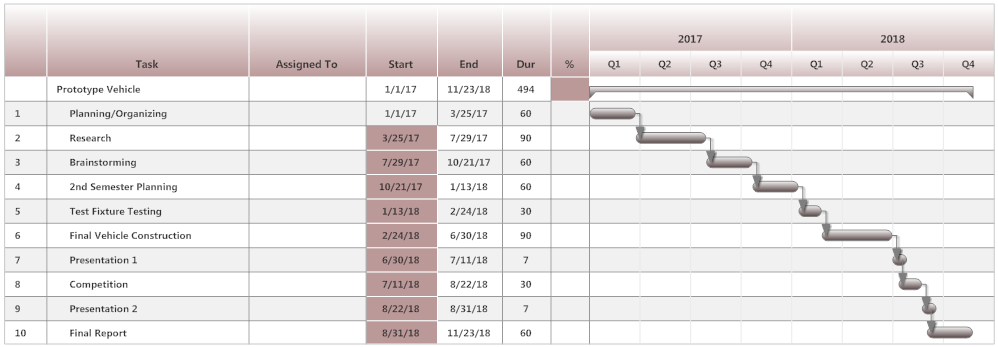
\includegraphics[width=\textwidth]{images/gantt2.png}
				\caption{Ein Gantt-Diagramm mit eingetragenem Critical Path. Von links nach rechts: Der Titel des Tasks, eine Spalte für den zugewiesenen Sachverständigen, Startdatum, Enddatum, Dauer, Anteil vervollständigt, grafische Darstellung der Tasks im Zeitplan mit eingetragenen Abhängigkeiten}
				\label{img:gantt}
			\end{center}
		\end{figure}
		Ein Gantt-Diagramm ist eine Visualisierung eines Projektablaufes, welche sowohl die Critical Path Method als auch PERT unterstüzt insofern als dass diese Techniken in die Erstellung eines Gantt-Diagramms eingebunden werden können.
		
		Bei Grafik \ref{img:gantt} ist die Einbindung des Critical Path in die Task-Visualisierung zu erkennen.
		Würden weitere Tasks zum Projekt hinzugefügt werden, würden diese nach Startdatum einsortiert werden, nachdem alle Abhängigkeiten mit eingeflossen sind.
		Hierbei ergeben sich mitunter Parallelisierungen von Tasks.
		
		\subsubsection{Erstellung eines Gantt-Diagramms.}
			\label{sssec:gantt-howto}
			Zunächst muss die Projektstruktur erfasst werden.
			Dies geschieht, indem die Ziele des Projektes klar definiert werden, anhand der Ziele Milestones genannt werden, und diese in überschaubare, spezifische Tasks aufgebrochen werden.
			Das Ziel muss dabei jedoch immer mit bedacht werden.
	
			Im nächsten Schritt werden die Aufgaben an die einzelnen Entwickler verteilt, dabei in Betracht ziehend, wer am Besten für eine bestimmte Aufgabe geeignet ist und wer zur Verfügung steht sowie Rücksicht nehmen auf die totale Arbeitslast der Mitarbeiter, sodass die Aufgaben gleichmäßig verteilt werden.
			
			Folgend wird für jeden Task die zu erwartende Dauer bestimmt.
			Hierbei kann mit der Formel von PERT vorgegangen werden, oder es wird nach Erfahrungswert eine Deadline gesetzt.
			
			Anschließend werden die Abhängigkeiten aufgelöst, sodass ersichtlich ist, welche Tasks wann erledigt werden müssen, um das Fortlaufen des Projektes zu gewährleisten.
			An dieser Stelle kann der Critical Path ermittelt werden.
			
			Zum Abschluss sollte das Diagramm dem Team vorgelegt werden, um Unstimmigkeiten aufzudecken.\footnote{
				https://www.smartdraw.com/gantt-chart/steps-to-managing-projects-with-gantt-charts.htm
			}
		\subsubsection{Vorteile.}
			\label{sssec:gantt-pro}
			Gantt-Diagramme erlauben das Sortieren von Projektdetails sowie das einfache Darstellen komplexer Zusammenhänge.
			Ebenso unterstützen sie bei der Erstellung, Einhaltung und Überarbeitung von Deadlines; auch Außenstehende können einen Überblick über den Projektstatus gewinnen.\footnote{
				http://www.pmhut.com/advantages-and-disadvantages-of-gantt-charts
			}
		\subsubsection{Nachteile.}
			\label{sssec:gantt-con}
			Wie jede Projektmanagementtechnik kann ein Gantt-Diagramm bei großen, komplexen Projekten unübersichtlich werden.
			Zudem muss es stets aktuell gehalten werden, jede Verschiebung im Zeitplan muss eingearbeitet werden.
			
			Die Darstellung kann große Ausmaße annehmen, weswegen sie zuweilen nicht auf einen Monitor passt und sich das Ausdrucken eines Diagramms als schwierig gestaltet.
			Ein großes Diagramm vorzuführen, ist somit ein aufwändiger Akt.
	
\section{Kurzzeitstrukturierung von Projekten}
	\label{sec:short-term}
	
	\subsection{Kanban}
		\label{ssec:kanban}
		\begin{figure}[ht]
			\begin{center}
				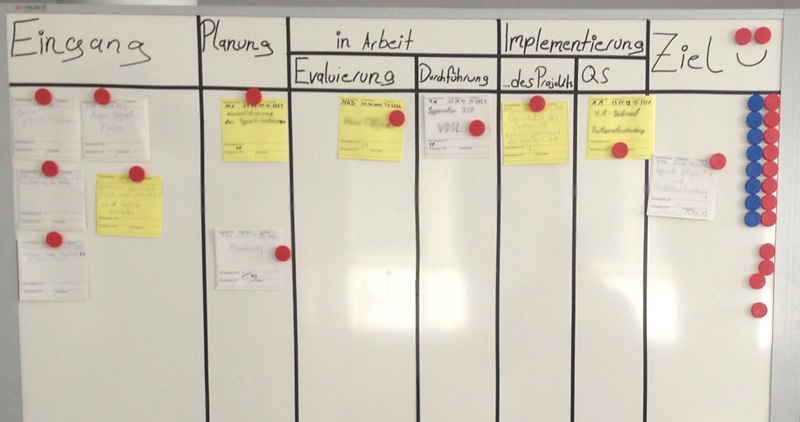
\includegraphics[width=\textwidth]{images/kanban-board.jpg}
				\caption{Kanban-Board mit den Kategorien \textit{Eingang}, \textit{Planung}, \textit{In Arbeit}, \textit{Implementierung} und \textit{Ziel}. \textit{In Arbeit} und \textit{Implementierung} sind jeweils aufgeteilt. Farben können zur Übermittlung von Informationen genutzt werden.}
				\label{img:kanban}
			\end{center}
		\end{figure}
		Kanban ist eine Praxis aus der Fertigungstechnik \textit{Lean}, entwickelt aus dem \textit{Toyota Production System}, welche zur Strukturierung und Übersicht von Tasks dient.
		Seine Ursprünge in der Automobilindustrie des Japans um den zweiten Weltkrieg habend, eignet sich Kanban dazu, auf effiziente Art und Weise neue Produkte zu fertigen, indem alles, was nicht mit der Produktion per se zu tun hat, wie unnötige Dokumentation oder Vorausproduktion gestrichen wird, und stattdessen on-Demand produziert wird, was analog zur agilen Entwicklung geht.
		
		Dabei wird in Phasen vorgegangen, welche keine Vorgaben und Zeitbeschränkung haben, sie können frei vom Team bestimmt werden.
		Generell gibt es aber einige Phasen, die immer oder meist vertreten sind.
		
		Die erste Phase, die sich auf fast jedem Kanban-Board findet, ist \textit{Eingang} oder \textit{Backlog}, in der alle Anforderungen aufgefangen und gesammelt werden.
		
		Ebenso ist meist eine Phase \textit{Planung} oder \textit{Todo} vorhanden, in der Tasks für die aktuelle Iteration gesammelt werden.
		
		\textit{In Arbeit} beziehungsweise \textit{Doing} sammelt alle Aufgaben, die derzeit bearbeitet werden.
		
		Nach Bedarf wird eine Spalte \textit{Review} oder \textit{QA} inseriert, bei der teaminternes Feedback zu vermeintlich abgeschlossenen Aufgaben angefordert wird.
		
		Zudem gibt es eine Phase \textit{Ziel}, \textit{Fertig}, \textit{Done} oder Ähnliches, in der alle fertigen Tasks gesammelt werden.
		
		Phasen werden traditionell in Spalten dargestellt, selten kann jedoch auch eine zeilenweise Darstellung vorgefunden werden.
		\-\\\\
		\addcontentsline{toc}{subsection}{todo}
		\begin{itemize}
			\item Visualisierung akuter Tasks
			\item Darstellung des Status des aktuellen Sprints
			\item Kategorisierbar und Bedingbar
		\end{itemize}
		\href{http://www.kanbansim.org/boards/b254f2363d0197a551180984b48b60a1}{Rumspielen?}
			
	\subsection{Daily Scrum und Stand-Up Meeting}
		\label{ssec:daily}
		Beide diese Aktionen werden von der agilen Welt als \textit{Daily Meeting} bezeichnet\footnote{
			\url{https://www.agilealliance.org/glossary/daily-meeting/}
		}.
		Das Stand-Up Meeting ist Teil des eXtreme Programming, das Daily Scrum kommt aus dem Scrum.
		Sie ähneln sich darin, dass sie täglich zur gleichen Zeit am gleichen Ort stattfinden und das ganze Team anwesend ist.
		Die Bezeichnung Stand-Up Meeting kommt daher, dass die Teilnehmer angehalten sind, während des ganzen Meetings zu stehen, um die Dauer möglichst gering und das Meeting kompakt und effizient zu halten.
		
		Der Daily Scrum orientiert sich an drei Leitfragen, um die Gespräche kontextnah zu halten\footnote{
			\url{https://www.agilealliance.org/glossary/three-qs/}
		}
		\begin{enumerate}
			\item Was wurde seit dem letzten Treffen fertig gestellt?
			\item Was soll bis zum nächsten Treffen theoretisch fertig sein?
			\item Welche Probleme sind aufgetreten?
		\end{enumerate}
		Auch im XP ist es nicht unüblich, diese Fragen während des Stand-Up Meeting zu beantworten.
		Ein Meeting wird generell mit einer Viertelstunde Zeitbedarf veranschlagt, kann jedoch bei größeren Teams auch länger dauern, und findet in der Regel vor einer Task-Übersicht wie dem Kanban-Brett statt.
		
		Der Begriff Daily Scrum wurde erstmals 1997 verwendet, 1998 wurde das Daily Stand-Up in die eXtreme Programming-Techniken aufgenommen, und 2000 wurden die drei Scrum-Fragen in eXtreme Programming eingegliedert.
		Um 2005 wurde es als Agile Kerntechnik angenommen.
		
		\subsubsection{Vorteile.}
			\label{sssec:daily-pro}
			Der Hauptvorteil ist, dass jedes Teammitglied alle relevanten Informationen sowie einen Überblick über den Projektstatus besitzt.
			Ebenso stärkt es den Zusammenhalt und die soziale Vernetzung im Team.
			Durch das Stehen sind die Treffen kürzer und effizienter als wenn das Team sitzen würde.
			Es kann jeden Tag kontrolliert werden, ob sich das Projekt noch in akzeptablen Parametern bewegt und welche Aufgaben als nächstes fällig sind.
			
		\subsubsection{Probleme.}
			\label{sssec:daily-con}
			Das Meeting sollte nach der Scrum-Philosophie mit allen Mitgliedern auf gleicher Ebene stattfinden, sodass es sich nicht um einen Statusbericht an den Teamleiter, sondern um ein Gespräch mit den Teammitgliedern handelt.
			
			Ein Meeting kann, sofern nicht regulierend eingegriffen wird, sehr in die Länge gezogen werden.
			Durch das Stehen soll dem ein wenig entgegengewirkt werden.
			
			Wenn Meetings zur Routine werden, ohne dass Motivation und Neuigkeiten vorhanden sind, droht das sogenannte \textit{Scrum Zombie}-Muster\footnote{
				\url{https://www.agilealliance.org/glossary/three-qs/}
			}, bei dem ein Mitarbeiter nur mitteilt, dass er an einem bestimmten Task gearbeitet habe, an einem neuen bestimmten Task arbeiten werde und keine Probleme aufgetreten seien.
			Dem kann entgegen gewirkt werden, indem eine klare Definition für erledigte Aufgaben gegeben wird.
			Desweiteren kann in solchen Situationen das Rederecht direkt weitergegeben werden\footnote{
				\url{https://www.agilealliance.org/glossary/three-qs/}
			}
			
		
\section{Softwareentwicklungsphilosophien}
	\label{sec:phil}
	\addcontentsline{toc}{subsection}{todo}
	Es wurden wiederholt zwei Philosophien angesprochen, die in der Softwareentwicklung Anwendung finden: Scrum und eXtreme Programming.
	
	Diese beiden Philosophien waren, wie schon eingangs erwähnt, maßgeblich, wenn auch nicht ausschließlich, an der Entstehung des Agilen Manifests beteiligt.
	
\section{Fazit}
	\label{sec:conclusion}
	\addcontentsline{toc}{subsection}{todo}
	Es wurde ein kurzer historischer Überblick über Softwareentwicklung gewonnen.
	Anschließend wurden modernere, heute verwendete Verfahren im Detail vorgestellt.
	Zum Abschluss wurden zwei Philosophien der Softwareentwicklung besprochen.
	
	In der Praxis ist es häufig so, dass ein Entwicklerteam nicht eine einzelne Technik anwendet oder einer einzelnen Philosophie folgt.
	Wie schon in Abschnitt \ref{ssec:gantt} angedeutet, werden Managementtechniken miteinander kombiniert, und Entwicklungstechniken passen sich laufend aneinander an, wie in \ref{ssec:daily} gezeigt.
	
	Eine gesunde Mischung ist die Verwendung von Sprints aus Scrum mit der Verbindung von Daily Stand-Ups aus XP und der Verwendung eines Kanban-Boards.
	Wenn es zu Beginn des Projektes bereits klare Zielvorgaben gibt, kann ein Gantt-Diagramm verwendet werden, um zusätzlich den Langzeitüberblick zu behalten.
	
	
\section*{Abbildungsverzeichnis}
	\addcontentsline{toc}{section}{Abbildungsverzeichnis}
	\begin{tabular}{r|p{.85\textwidth}}
		\textbf{Nummer}		&	\textbf{Quelle}	\\ \hline
		
		\ref{img:waterfall}	&	\textbf{Grafik:} \url{http://www.oxagile.com/wp-content/uploads/2014/02/waterfall.png},
								\textbf{Seite:} \url{http://www.oxagile.com/company/blog/the-waterfall-model/}	\\\hline
		\ref{img:crit}		&	\textbf{Grafik:} \url{http://tr1.cbsistatic.com/hub/i/2009/09/09/76bb5c08-c3b4-11e2-bc00-02911874f8c8/cpm1.jpg},
								\textbf{Seite:} \url{http://www.techrepublic.com/blog/tech-decision-maker/why-critical-path-is-critical-to-project-management/}	\\\hline
		\ref{img:pert}		&	\textbf{Grafik:} \url{https://upload.wikimedia.org/wikipedia/commons/thumb/3/37/Pert_chart_colored.svg/1000px-Pert_chart_colored.svg.png},
								\textbf{Seite:}	 \url{https://en.wikipedia.org/wiki/Program_evaluation_and_review_technique}\\\hline
		\ref{img:gantt}		&	\textbf{Grafik:} \url{https://wcs.smartdraw.com/cmsstorage/exampleimages/49d69987-97a4-4d57-8123-262e16a32261.png?bn=1510011143},
								\textbf{Seite:} \url{https://www.smartdraw.com/gantt-chart/examples/prototype-vehicle-gantt-chart/}	\\\hline
		\ref{img:kanban}	&	\textbf{Grafik:} \url{http://blog.novatec-gmbh.de/wp-content/uploads/2013/05/kanban-board.jpg}, 
	
	\end{tabular}

\section*{Quellenverzeichnis}
	\addcontentsline{toc}{section}{Quellenverzeichnis}
	
	
	


%%% Local Variables: 
%%% mode: latex
%%% TeX-master: "main"
%%% End: 


%\bibliographystyle{gerplain}
\bibliographystyle{plain}
%% add your temporary bib file here (white spaces do not work)
%%\bibliography{../defs,../cap,mynamebib} 
\bibliography{../defs,../aose} 
\printindex

\end{document}





%%% Local Variables: 
%%% mode: latex
%%% TeX-master: "main"
%%% End: 
